\documentclass{article}
\usepackage{graphicx} % Required for inserting images

%\documentclass[a4paper,12pt]{article}
\usepackage{amsmath}
\usepackage{graphicx}
\usepackage{hyperref}
\usepackage{url}
\usepackage[finnish]{babel}
\usepackage{attachfile}

\title{PT-100 palautus}
\author{Elias Myllymäki}
% \date{March 2025}

\begin{document}

\maketitle

% \section{Introduction}






\section*{Tehtävä 1}

\subsection*{A)}
18 ohmin vastus $\pm 5\%$, mitattu arvo 17,9 ohmia, mittausalue 600 ohmia.

\subsection*{B)}
Sininen vastus 10 megaohmia $\pm 1\%$, mitattu arvo 10,01 megaohmia, mittausalue 100 megaohmia.

\subsection*{C)}
Mittausalue valitsee arvoalueen, jota mitataan. Se vaikuttaa mittauksen herkkyyteen ja virheeseen. 
Päädyimme käyttämään näitä mittausalueita, koska oskilloskooppi automaattisesti sääti ne meille.
Emme kokeilleet manuaalisesti vääriä mittausalueita, mutta jos olisimme, niin liian isolla mittausalueella 
mittaukset olisivat olleet epätarkkoja, ja liian pienellä mittausalueella mittaus ei onnistuisi, 
koska arvot hyppisivät mittausalueelta pois (\textit{clipping}).

\section*{Tehtävä 2}

\subsection*{A)}
Mittausdata oli CSV (\textit{comma separated values}) -tiedostossa. 
Tämän voi avata esimerkiksi Excelillä, Google Sheetsilla tai Pythonilla.

\subsection*{B)}
CSV-tiedosto sisälsi metadataa (mittauslaitteen sarjanumeron ja mallin) sekä vastusmittaukset 
ja mittausajat sekunteina mittauksen alusta.

Tiedoston otsake oli seuraavanlainen:

\begin{verbatim}
Serial number:,23380892
Function:,RES,Unit:,Ω
Start date:,2024/10/25,Start time:,20:00:14
Sample:,1.000s
Reading #,Reading
\end{verbatim}

Jonka jälkeen itse mittausdata oli. Laitteen sisäinen kello on väärässä, koska se väittää olevansa vuodessa 2024, 
vaikka oikeasti oli vuosi 2025, kun mittaukset tehtiin.

\subsection*{C)}
Alla on kuvaaja kuvassa 1.
\begin{figure}[!h]
    \centering
    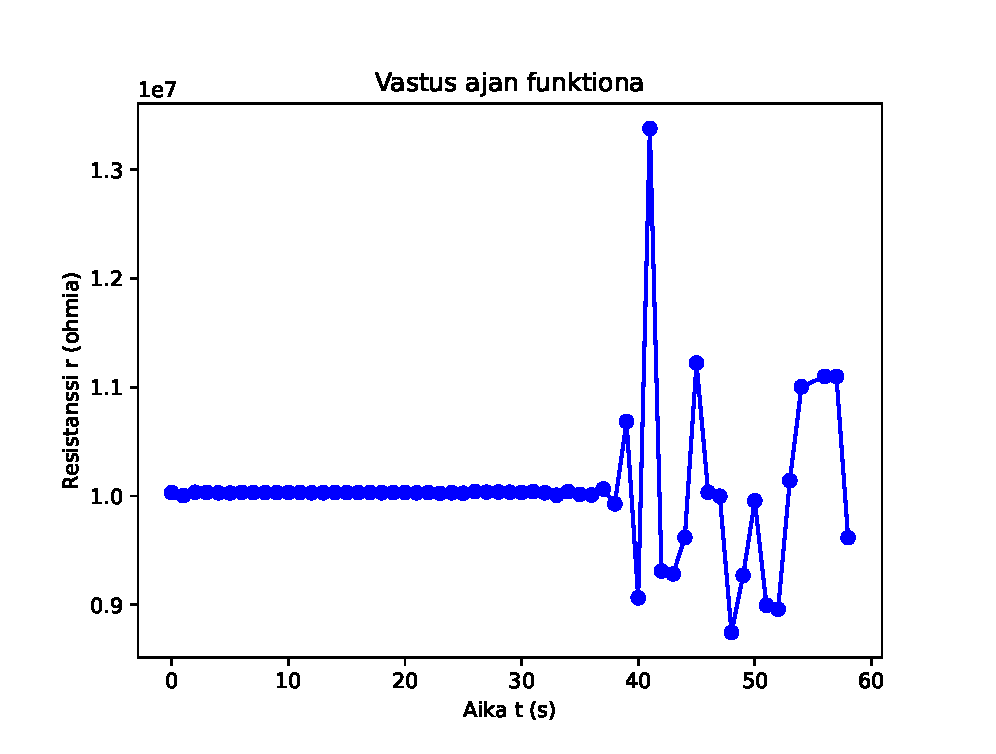
\includegraphics[width=1.0\linewidth]{hairio_plot.eps}
    \caption{Vastus ajan funktiona. Noin 30s kohdalla koejärjestelyä alettiin siirrellä.}
    \label{fig:hairio_plotting}
\end{figure}

\subsection*{D)}

ei.

\subsection*{E)}
Tärähdykset vaikuttavat mittauslaitteen ja mitatun komponentin väliseen liitokseen siten, 
että sen vastus vaihtelee.

\section*{Tehtävä 3}

\subsection*{A)}
Resistanssi nousee noin ohmilla.

\subsection*{B)}
PT-100:n vastus nousee lämpötilan noustessa. Tämä johtuu siitä, että metallihila heiluu lämmön vaikutuksesta, 
ja se vaikeuttaa elektronien kulkemista. \cite{therma_temperature_resistance}

Sanotaan, että platinassa lämpötilan noustessa fononitörmäykset lisääntyvät. 
\cite{wikipedia_phonon_scattering}

\subsection*{C)}
Malli PT-100-vastuksen lämpötilariippuvuudelle on:

\[
R_{(T)} = R_{(0)} \cdot \left( 1 + a \cdot T + b \cdot T^2 \right)
\]
eli
\[
T = \frac{-a \pm \sqrt{a^2 - 4b(1 - k)}}{2b}
\]
missä $k = \frac{R_{(T)}}{R_{(0)}}$
Missä $R_{(0)}$ on vastus 0°C:ssa, joka on määritelty sadaksi ohmiksi.
Vakio $a = 3.9083 \times 10^{-3}$ ja vakio $b = -5.775 \times 10^{-7}.$. Tästä yhtälöstä käytämme vain positiivista juurta.

\subsection*{D)}

Arvot vastuksille on otettu datasta. Datan mukaan laboratorion lämpötila oli noin $20,53\,^\circ \text{C}$

\subsection*{E)}

Alla kuvassa 2 kuvaaja

\begin{figure}[h!]
    \centering
    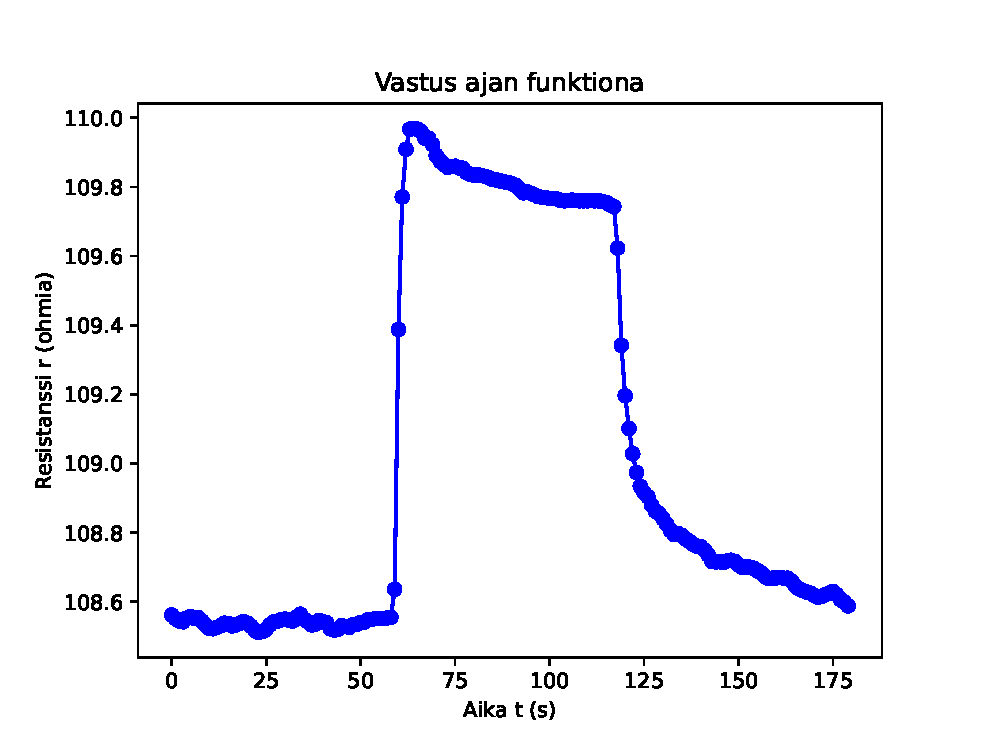
\includegraphics[width=1.0\linewidth]{resistance_plot.eps}
    \caption{Vastus ajan funktiona}
    \label{fig:resistance_plot_figure}
\end{figure}
\newpage
\subsection*{F)}
Vakioitui nopeammin sormien lämpötilaan, koska kuvaajan mukaan siihen kesti vain noin 25 sekuntia, kun taas takaisin huoneenlämpöön siihen kesti noin 50 sekuntia.
\subsection*{G)}
Noin $25,7\,^\circ\text{C}$ . Tämä ei vastaa ihmisen ruumiinlämpötilaa, mutta tämä on odotettavissa, koska lämpötila raajojen äärissä on eri kuin keskellä kehoa. Raajojen lämpötila riippuu tietenkin vuorostaan ympäristön lämpötilasta.

\section*{Tehtävä 4}

Harjoituksessa oli erityisen vaikeaa pöytämultimittarin käyttö, 
koska se ei havainnut USB-tikkua melkein ikinä, vaan oli täysin sattumanvaraista, 
milloin se "huomasi" (recognize) sen ja milloin ei.

\bibliographystyle{plain}
\bibliography{sources}

\section*{Liitteet}
Tässä tiedostossa on liitetty kaikki lähdekooditiedostot ja raaka mittausdata tiedostona 'allfiles.zip'. Voit purkaa tämän esimerkiksi 'pdfdetach' työkalulla. Tämän lisäksi lähdekoodi on myös minun github sivullani \url{https://github.com/personnumber3377/pt100} \attachfile{sources.bib}


\end{document}
